While our default threaded allocator performs and scales well, we also explored
some alternative designs. In this section, we explore a design where we move the
allocation decisions from the thread to the node itself, in order to store the
facts of the same node close together and thus increase locality. However, this
design requires locking since multiple threads may allocate facts from the same
node. Our expectation is that such costs will be offset by the increased
locality and reduced cache misses when deriving rules.

The fact allocator allocates pages of memory from the threaded allocator which
are then used to allocate facts for that particular node. When a thread needs to
allocate or deallocate a fact, it acquires the allocator lock of the target
node's allocator and performs the allocation operation. There is a doubly-linked
list of memory pages and each page contains facts of different sizes
(predicates).

\begin{figure}[ht]
   \begin{center}
      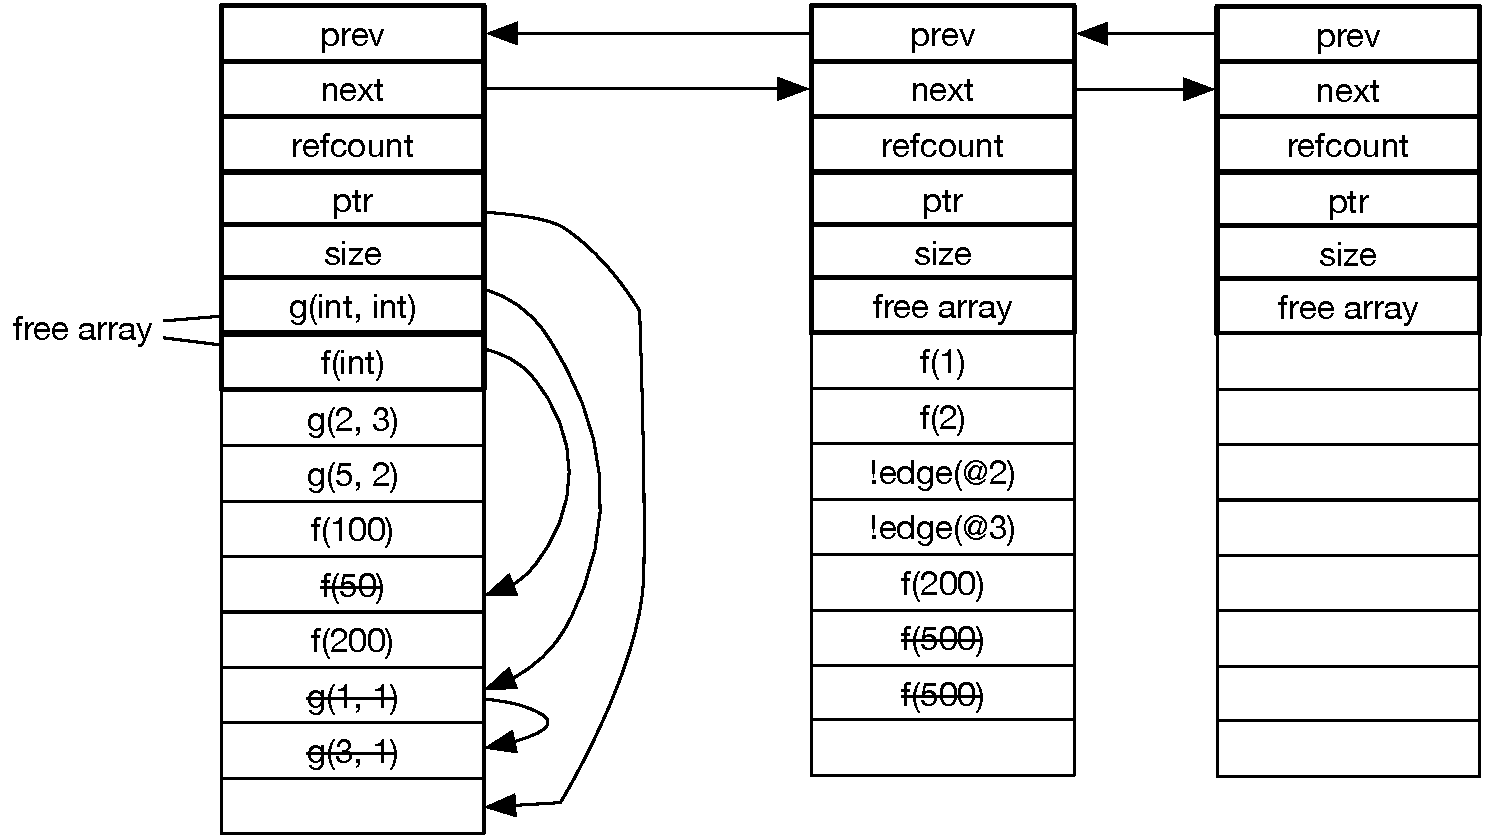
\includegraphics[width=0.7\linewidth]{figures/implementation/fact_allocator.pdf}
   \end{center}

   \mycap{Fact allocator: each node has a pool of memory pages for allocating
      logical facts. Each page contains: (i) several linked lists of free facts
      of the same size (\code{free\_array}); (ii) a reference count of used
      facts (\code{refcount}); (iii) a \code{ptr} pointer that points to
      unallocated space in the page. In this figure, predicates \code{f} and
      \code{g} have several deallocated facts that are ready to be used when a
   new fact needs to be acquired.}

   \label{fig:implementation:fact_allocator}
\end{figure}

Figure~\ref{fig:implementation:fact_allocator} presents an example state of a
fact allocator. The node has 3 memory pages, all connected using the \code{next}
and \code{prev} pointers. Each page also has a reference count (\code{refcount})
of the objects allocated in the page. If the reference count ever drops to zero,
then the memory page is deallocated. Deallocated facts are kept on an ordered
array for different sizes using the mechanism we implemented for the threaded
allocator. We have decided to reference count objects in the fact allocator
because it is more difficult to share objects between nodes and maintaining a
reference count helps reduce memory usage.

Figure~\ref{fig:implementation:node_results} presents the comparison between the
threaded and fact allocator for the most relevant datasets (the performance was
similar for the other datasets).

\begin{figure}[h]
        \begin{subfigure}[b]{\smallplotsize\textwidth}
                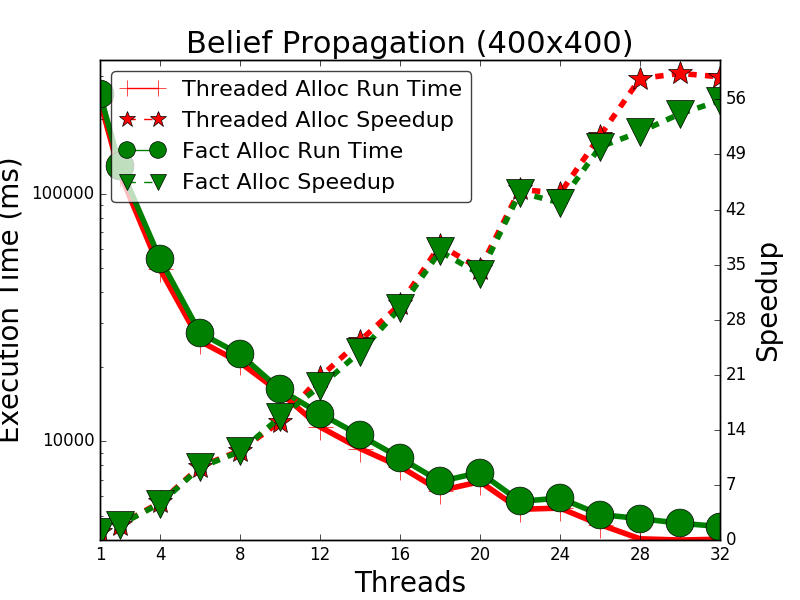
\includegraphics[width=\textwidth]{experiments/scalability/node-allocator-belief-propagation-400.png}
                \label{fig:implementation:node_bp}
        \end{subfigure}
        ~
        \begin{subfigure}[b]{\smallplotsize\textwidth}
                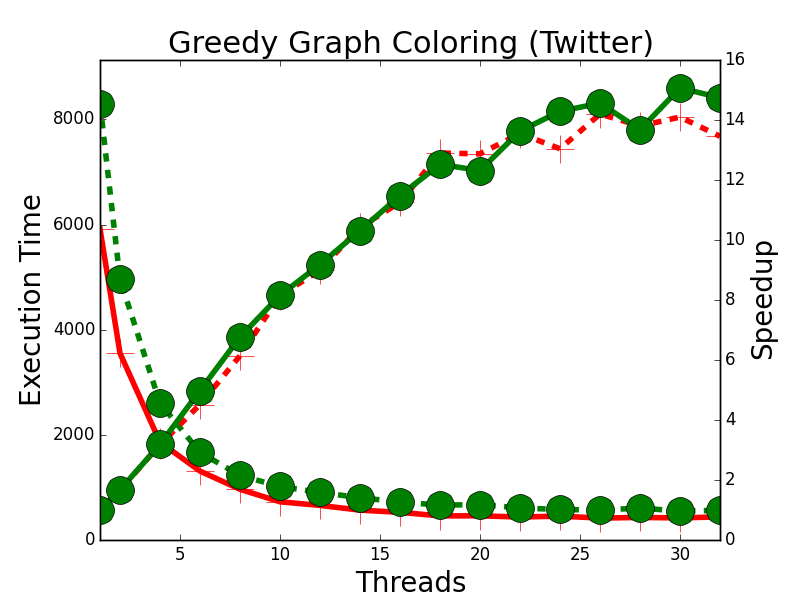
\includegraphics[width=\textwidth]{experiments/scalability/node-allocator-greedy-graph-coloring-twitter.png}
                \label{fig:implementation:node_ggc}
        \end{subfigure}
        ~
        \begin{subfigure}[b]{\smallplotsize\textwidth}
                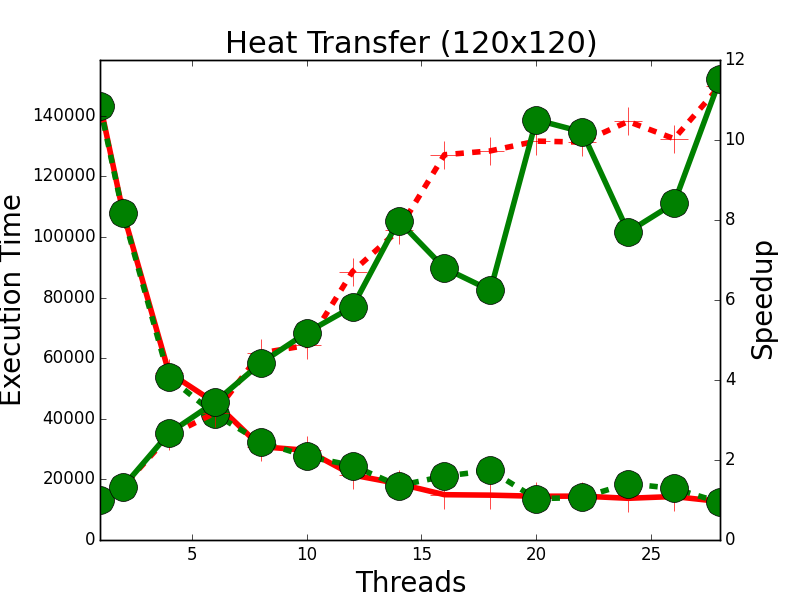
\includegraphics[width=\textwidth]{experiments/scalability/node-allocator-new-heat-transfer-120.png}
                \label{fig:implementation:node_ht}
        \end{subfigure}
        ~
        \begin{subfigure}[b]{\smallplotsize\textwidth}
                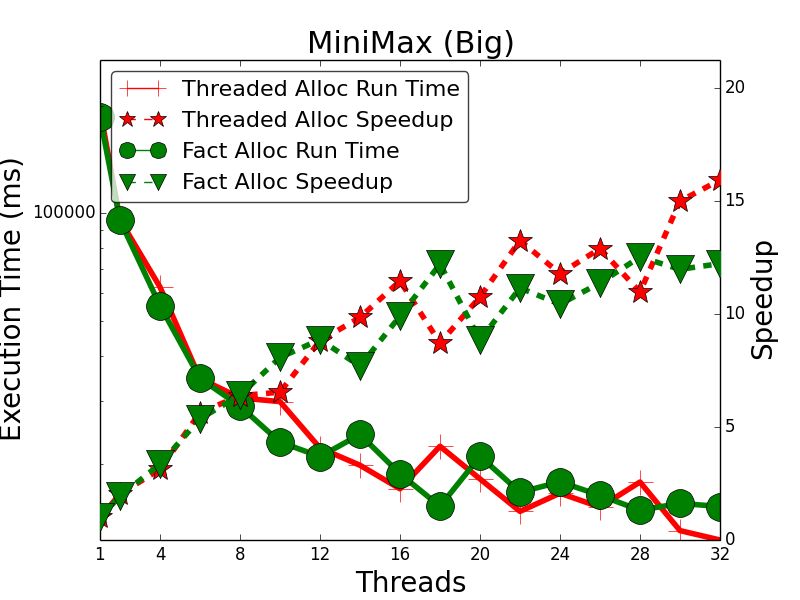
\includegraphics[width=\textwidth]{experiments/scalability/node-allocator-min-max-tictactoe-big.png}
                \label{fig:implementation:node_minimax}
        \end{subfigure}
        ~
        \begin{subfigure}[b]{\smallplotsize\textwidth}
                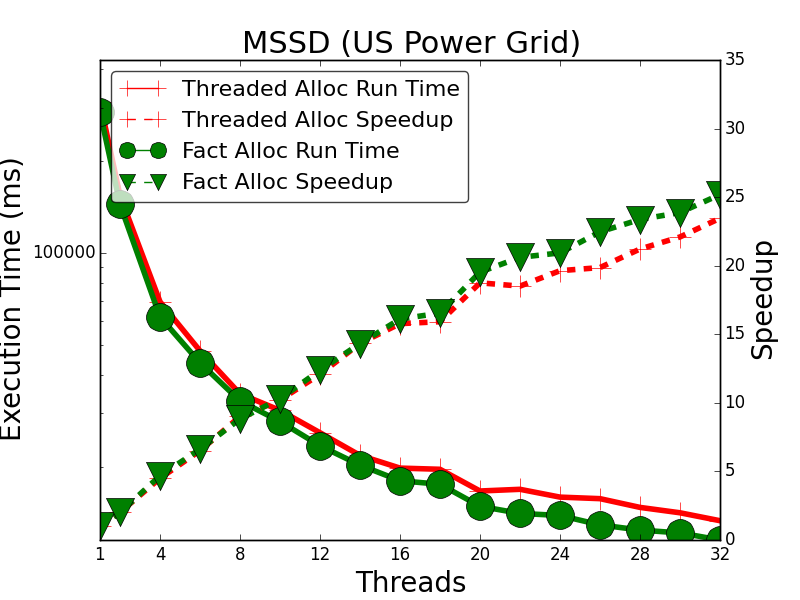
\includegraphics[width=\textwidth]{experiments/scalability/node-allocator-shortest-uspowergrid.png}
                \label{fig:implementation:node_sssp}
        \end{subfigure}
        ~
        \begin{subfigure}[b]{\smallplotsize\textwidth}
                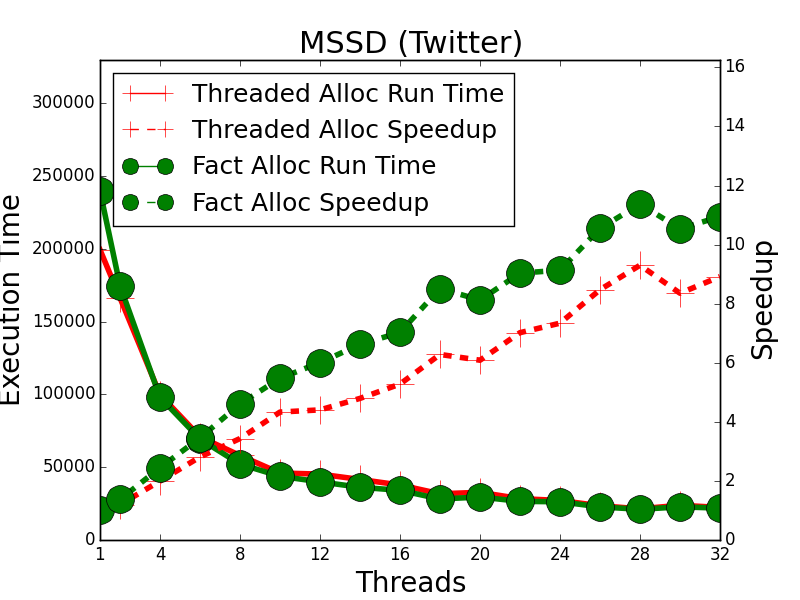
\includegraphics[width=\textwidth]{experiments/scalability/node-allocator-shortest-twitter.png}
                \label{fig:implementation:node_sssp}
        \end{subfigure}\\
        \begin{subfigure}[b]{\smallplotsize\textwidth}
                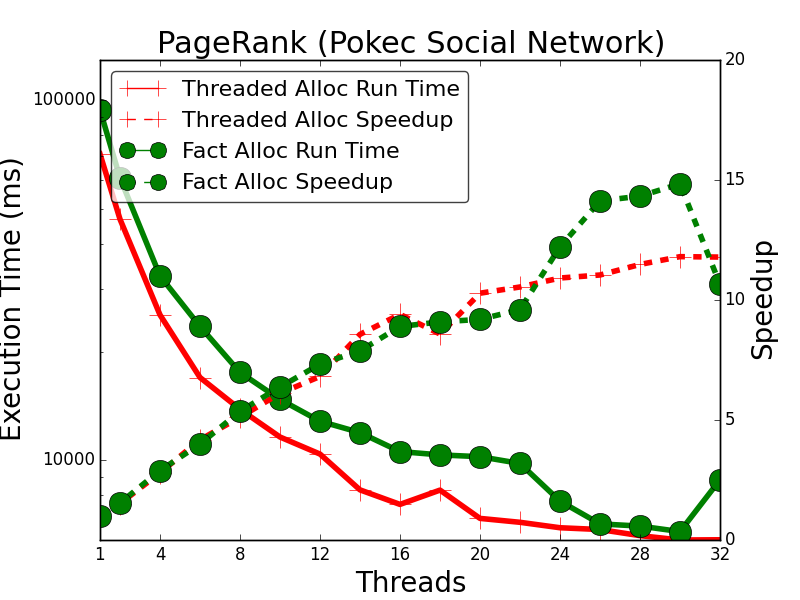
\includegraphics[width=\textwidth]{experiments/scalability/node-allocator-pagerank-pokec.png}
                \label{fig:implementation:node_pagerank}
        \end{subfigure}
        ~
        \begin{subfigure}[b]{\smallplotsize\textwidth}
                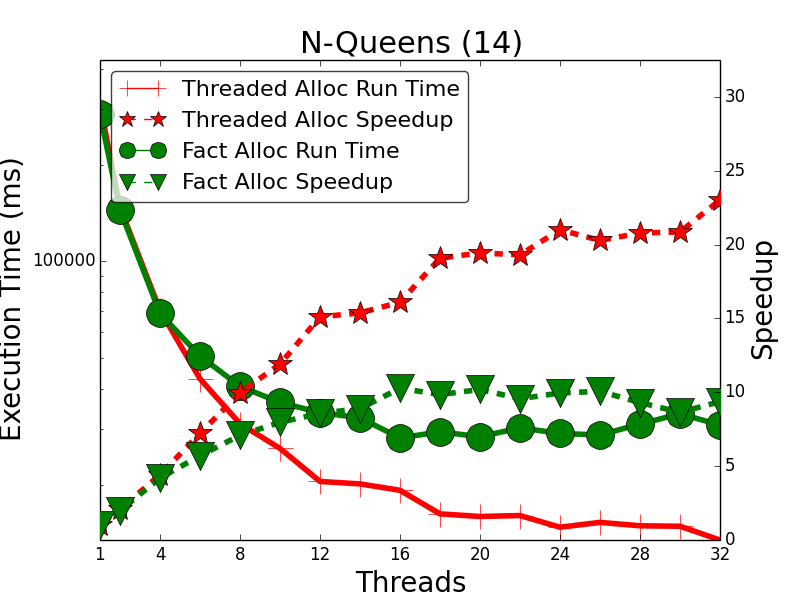
\includegraphics[width=\textwidth]{experiments/scalability/node-allocator-8queens-14.png}
                \label{fig:implementation:node_queens}
        \end{subfigure} \\
        \mycap{Comparing the threaded allocator described in
        Section~\ref{section:implementation:allocation} against the fact
     allocator.}

        \label{fig:implementation:node_results}
\end{figure}

The first major observation from the comparison is that the threaded allocator
has better sequential performance than the fact allocator for most programs.
This is probably the result of better locality for the threaded allocator
because it does not need to create pages for each node and instead uses the
thread pages to maintain all facts, reducing cache line misses. Overall, the
performance of the threaded allocator is better or similar than the fact
allocator, for both single and multithreaded threaded execution (see GGC for a
clear example).

The second observation is in the N-Queens program, where the threaded allocator
beats the fact allocator by a high margin in terms of scalability and
performance. Note that the N-Queens program allocates many of lists and those
lists are not allocated on a per node basis but on a thread basis, therefore the
extra work required to maintain each fact allocator is not offset by the
increased locality because the threads need to traverse lists to find valid
board states.

To make our comparison more interesting, we also deactivated the reference
counting mechanisms of the fact allocator and compared it against the threaded
allocator. The goal is to understand how reference counting affects the
performance of the alternative allocator. The complete comparison are shown in
Fig.~\ref{fig:implementation:no_refs_results}. In a nutshell, it performs almost
the same as the full featured fact allocator, except for programs which require
more memory such as MiniMax and Heat Transfer. In the case of MiniMax, we were
unable to completely execute the Big dataset since the VM required more memory
than the available memory, resulting in long execution times. This is the result
of not collecting unused memory pages, which results in high memory usage.


\begin{figure}[h]
        \begin{subfigure}[b]{\smallplotsize\textwidth}
                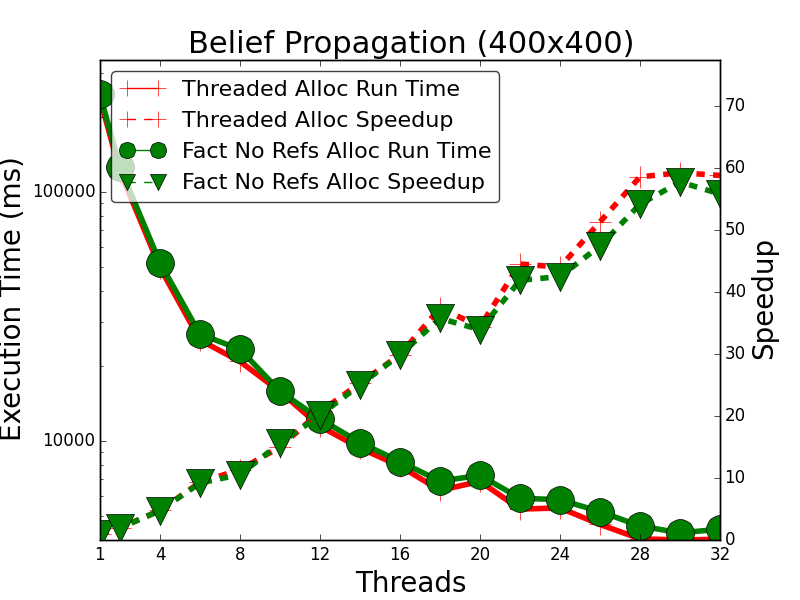
\includegraphics[width=\textwidth]{experiments/scalability/no-refs-allocator-belief-propagation-400.png}
                \label{fig:implementation:no_refs_bp}
        \end{subfigure}
        ~
        \begin{subfigure}[b]{\smallplotsize\textwidth}
                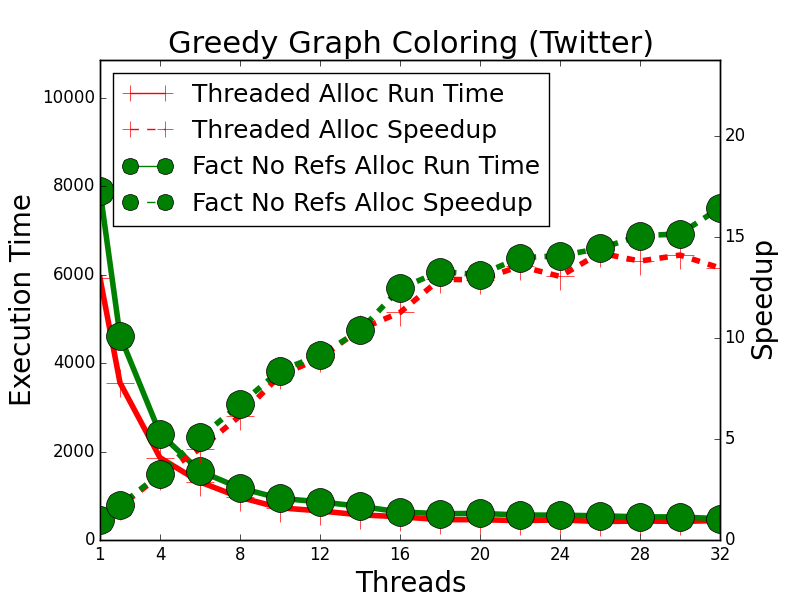
\includegraphics[width=\textwidth]{experiments/scalability/no-refs-allocator-greedy-graph-coloring-twitter.png}
                \label{fig:implementation:no_refs_ggc}
        \end{subfigure}
        ~
        \begin{subfigure}[b]{\smallplotsize\textwidth}
                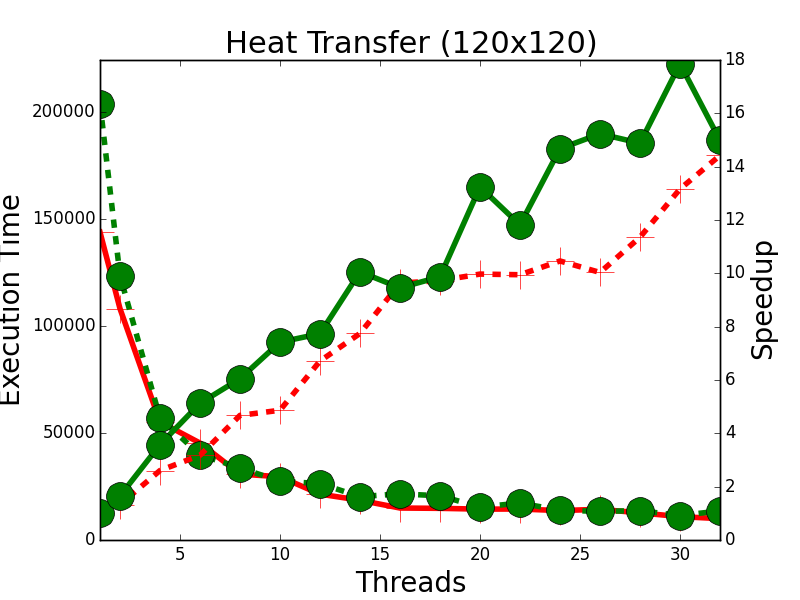
\includegraphics[width=\textwidth]{experiments/scalability/no-refs-allocator-new-heat-transfer-120.png}
                \label{fig:implementation:no_refs_ht}
        \end{subfigure}
        ~
        \begin{subfigure}[b]{\smallplotsize\textwidth}
                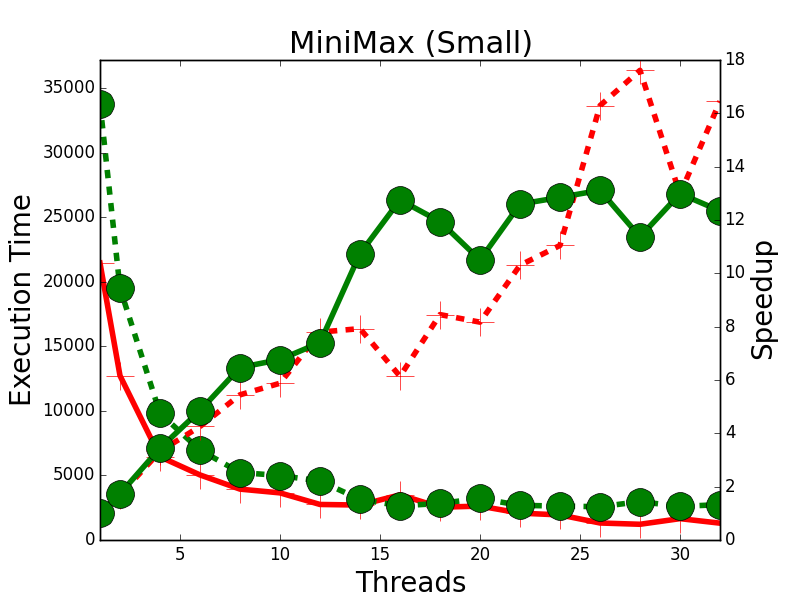
\includegraphics[width=\textwidth]{experiments/scalability/no-refs-allocator-min-max-tictactoe-small.png}
                \label{fig:implementation:no_refs_minimax}
        \end{subfigure}
        ~
        \begin{subfigure}[b]{\smallplotsize\textwidth}
                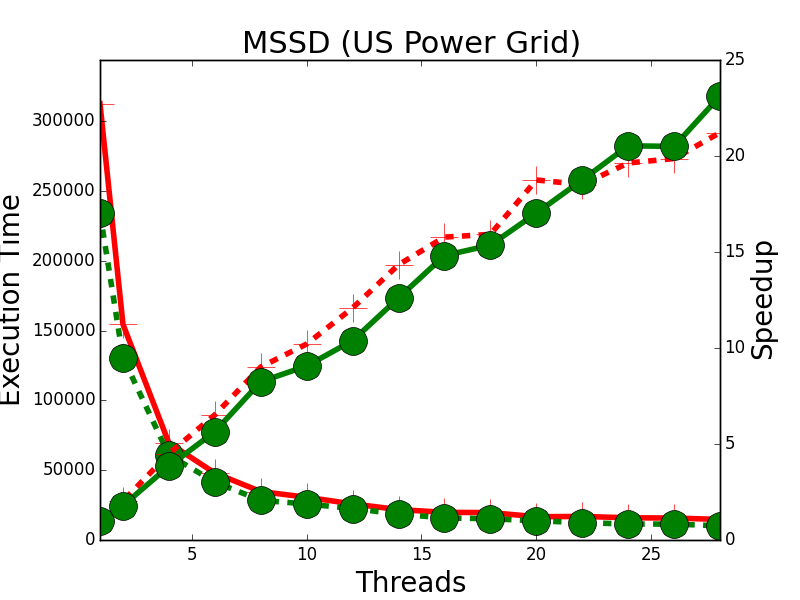
\includegraphics[width=\textwidth]{experiments/scalability/no-refs-allocator-shortest-uspowergrid.png}
                \label{fig:implementation:no_refs_sssp}
        \end{subfigure}
        ~
        \begin{subfigure}[b]{\smallplotsize\textwidth}
                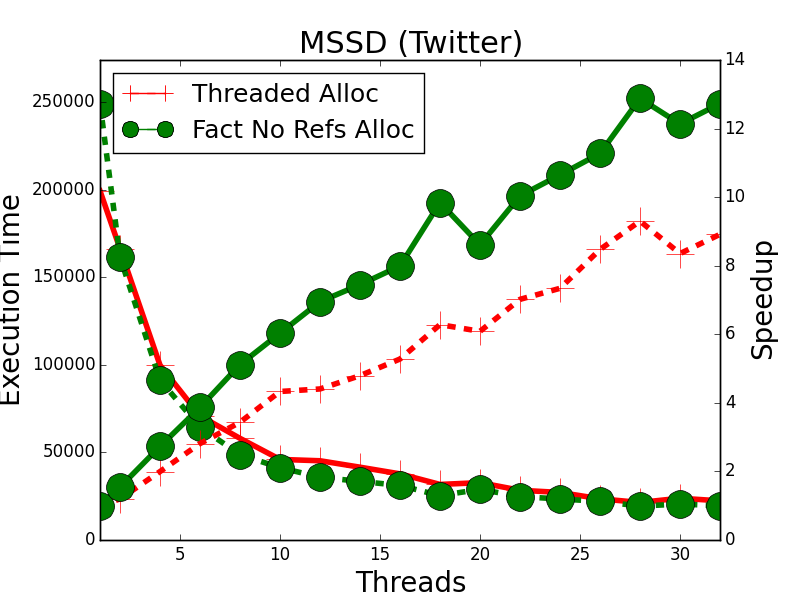
\includegraphics[width=\textwidth]{experiments/scalability/no-refs-allocator-shortest-twitter.png}
                \label{fig:implementation:no_refs_sssp2}
        \end{subfigure}\\
        \begin{subfigure}[b]{\smallplotsize\textwidth}
                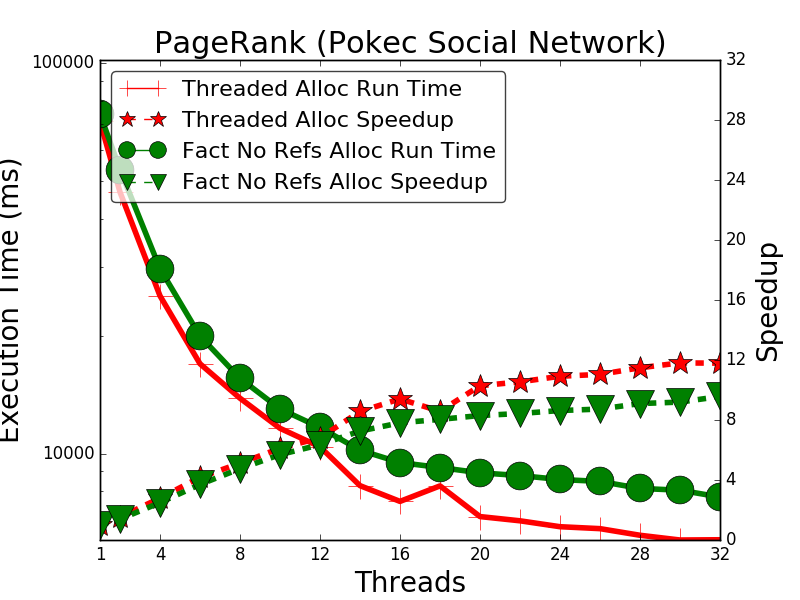
\includegraphics[width=\textwidth]{experiments/scalability/no-refs-allocator-pagerank-pokec.png}
                \label{fig:implementation:no_refs_pagerank}
        \end{subfigure}
        ~
        \begin{subfigure}[b]{\smallplotsize\textwidth}
                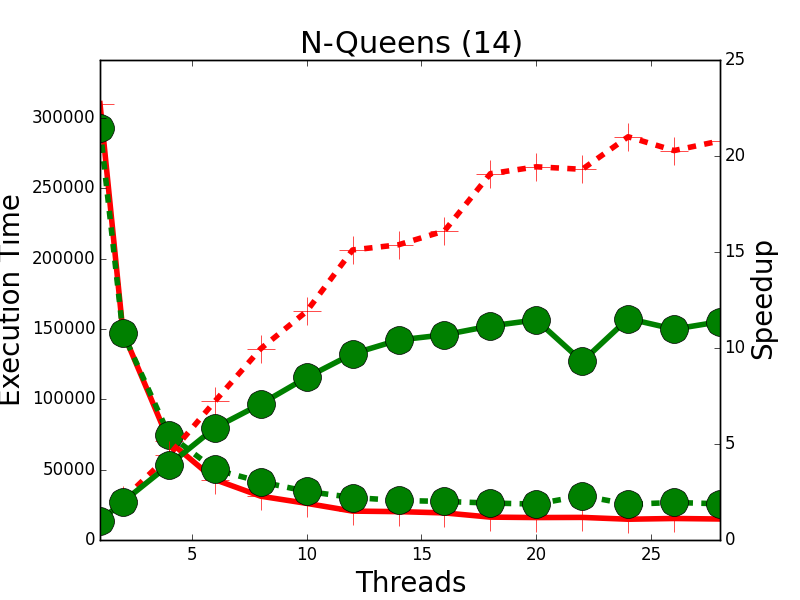
\includegraphics[width=\textwidth]{experiments/scalability/no-refs-allocator-8queens-14.png}
                \label{fig:implementation:no_refs_queens}
        \end{subfigure} \\

        \mycap{Comparing the threaded allocator described in
           Section~\ref{section:implementation:allocation} against the fact
        allocator without reference counting.}

        \label{fig:implementation:no_refs_results}
\end{figure}


Overall, the performance of both allocators is similar, therefore we have
decided to use the threaded allocator by default since it is simpler and offers
good performance across the board. Furthermore, the threaded allocator requires
less allocated memory because it enables more sharing between nodes.

